% Options for packages loaded elsewhere
\PassOptionsToPackage{unicode}{hyperref}
\PassOptionsToPackage{hyphens}{url}
\PassOptionsToPackage{dvipsnames,svgnames,x11names}{xcolor}
%
\documentclass[
  letterpaper,
  DIV=11,
  numbers=noendperiod]{scrreprt}

\usepackage{amsmath,amssymb}
\usepackage{iftex}
\ifPDFTeX
  \usepackage[T1]{fontenc}
  \usepackage[utf8]{inputenc}
  \usepackage{textcomp} % provide euro and other symbols
\else % if luatex or xetex
  \usepackage{unicode-math}
  \defaultfontfeatures{Scale=MatchLowercase}
  \defaultfontfeatures[\rmfamily]{Ligatures=TeX,Scale=1}
\fi
\usepackage{lmodern}
\ifPDFTeX\else  
    % xetex/luatex font selection
\fi
% Use upquote if available, for straight quotes in verbatim environments
\IfFileExists{upquote.sty}{\usepackage{upquote}}{}
\IfFileExists{microtype.sty}{% use microtype if available
  \usepackage[]{microtype}
  \UseMicrotypeSet[protrusion]{basicmath} % disable protrusion for tt fonts
}{}
\makeatletter
\@ifundefined{KOMAClassName}{% if non-KOMA class
  \IfFileExists{parskip.sty}{%
    \usepackage{parskip}
  }{% else
    \setlength{\parindent}{0pt}
    \setlength{\parskip}{6pt plus 2pt minus 1pt}}
}{% if KOMA class
  \KOMAoptions{parskip=half}}
\makeatother
\usepackage{xcolor}
\setlength{\emergencystretch}{3em} % prevent overfull lines
\setcounter{secnumdepth}{5}
% Make \paragraph and \subparagraph free-standing
\makeatletter
\ifx\paragraph\undefined\else
  \let\oldparagraph\paragraph
  \renewcommand{\paragraph}{
    \@ifstar
      \xxxParagraphStar
      \xxxParagraphNoStar
  }
  \newcommand{\xxxParagraphStar}[1]{\oldparagraph*{#1}\mbox{}}
  \newcommand{\xxxParagraphNoStar}[1]{\oldparagraph{#1}\mbox{}}
\fi
\ifx\subparagraph\undefined\else
  \let\oldsubparagraph\subparagraph
  \renewcommand{\subparagraph}{
    \@ifstar
      \xxxSubParagraphStar
      \xxxSubParagraphNoStar
  }
  \newcommand{\xxxSubParagraphStar}[1]{\oldsubparagraph*{#1}\mbox{}}
  \newcommand{\xxxSubParagraphNoStar}[1]{\oldsubparagraph{#1}\mbox{}}
\fi
\makeatother

\usepackage{color}
\usepackage{fancyvrb}
\newcommand{\VerbBar}{|}
\newcommand{\VERB}{\Verb[commandchars=\\\{\}]}
\DefineVerbatimEnvironment{Highlighting}{Verbatim}{commandchars=\\\{\}}
% Add ',fontsize=\small' for more characters per line
\usepackage{framed}
\definecolor{shadecolor}{RGB}{241,243,245}
\newenvironment{Shaded}{\begin{snugshade}}{\end{snugshade}}
\newcommand{\AlertTok}[1]{\textcolor[rgb]{0.68,0.00,0.00}{#1}}
\newcommand{\AnnotationTok}[1]{\textcolor[rgb]{0.37,0.37,0.37}{#1}}
\newcommand{\AttributeTok}[1]{\textcolor[rgb]{0.40,0.45,0.13}{#1}}
\newcommand{\BaseNTok}[1]{\textcolor[rgb]{0.68,0.00,0.00}{#1}}
\newcommand{\BuiltInTok}[1]{\textcolor[rgb]{0.00,0.23,0.31}{#1}}
\newcommand{\CharTok}[1]{\textcolor[rgb]{0.13,0.47,0.30}{#1}}
\newcommand{\CommentTok}[1]{\textcolor[rgb]{0.37,0.37,0.37}{#1}}
\newcommand{\CommentVarTok}[1]{\textcolor[rgb]{0.37,0.37,0.37}{\textit{#1}}}
\newcommand{\ConstantTok}[1]{\textcolor[rgb]{0.56,0.35,0.01}{#1}}
\newcommand{\ControlFlowTok}[1]{\textcolor[rgb]{0.00,0.23,0.31}{\textbf{#1}}}
\newcommand{\DataTypeTok}[1]{\textcolor[rgb]{0.68,0.00,0.00}{#1}}
\newcommand{\DecValTok}[1]{\textcolor[rgb]{0.68,0.00,0.00}{#1}}
\newcommand{\DocumentationTok}[1]{\textcolor[rgb]{0.37,0.37,0.37}{\textit{#1}}}
\newcommand{\ErrorTok}[1]{\textcolor[rgb]{0.68,0.00,0.00}{#1}}
\newcommand{\ExtensionTok}[1]{\textcolor[rgb]{0.00,0.23,0.31}{#1}}
\newcommand{\FloatTok}[1]{\textcolor[rgb]{0.68,0.00,0.00}{#1}}
\newcommand{\FunctionTok}[1]{\textcolor[rgb]{0.28,0.35,0.67}{#1}}
\newcommand{\ImportTok}[1]{\textcolor[rgb]{0.00,0.46,0.62}{#1}}
\newcommand{\InformationTok}[1]{\textcolor[rgb]{0.37,0.37,0.37}{#1}}
\newcommand{\KeywordTok}[1]{\textcolor[rgb]{0.00,0.23,0.31}{\textbf{#1}}}
\newcommand{\NormalTok}[1]{\textcolor[rgb]{0.00,0.23,0.31}{#1}}
\newcommand{\OperatorTok}[1]{\textcolor[rgb]{0.37,0.37,0.37}{#1}}
\newcommand{\OtherTok}[1]{\textcolor[rgb]{0.00,0.23,0.31}{#1}}
\newcommand{\PreprocessorTok}[1]{\textcolor[rgb]{0.68,0.00,0.00}{#1}}
\newcommand{\RegionMarkerTok}[1]{\textcolor[rgb]{0.00,0.23,0.31}{#1}}
\newcommand{\SpecialCharTok}[1]{\textcolor[rgb]{0.37,0.37,0.37}{#1}}
\newcommand{\SpecialStringTok}[1]{\textcolor[rgb]{0.13,0.47,0.30}{#1}}
\newcommand{\StringTok}[1]{\textcolor[rgb]{0.13,0.47,0.30}{#1}}
\newcommand{\VariableTok}[1]{\textcolor[rgb]{0.07,0.07,0.07}{#1}}
\newcommand{\VerbatimStringTok}[1]{\textcolor[rgb]{0.13,0.47,0.30}{#1}}
\newcommand{\WarningTok}[1]{\textcolor[rgb]{0.37,0.37,0.37}{\textit{#1}}}

\providecommand{\tightlist}{%
  \setlength{\itemsep}{0pt}\setlength{\parskip}{0pt}}\usepackage{longtable,booktabs,array}
\usepackage{calc} % for calculating minipage widths
% Correct order of tables after \paragraph or \subparagraph
\usepackage{etoolbox}
\makeatletter
\patchcmd\longtable{\par}{\if@noskipsec\mbox{}\fi\par}{}{}
\makeatother
% Allow footnotes in longtable head/foot
\IfFileExists{footnotehyper.sty}{\usepackage{footnotehyper}}{\usepackage{footnote}}
\makesavenoteenv{longtable}
\usepackage{graphicx}
\makeatletter
\def\maxwidth{\ifdim\Gin@nat@width>\linewidth\linewidth\else\Gin@nat@width\fi}
\def\maxheight{\ifdim\Gin@nat@height>\textheight\textheight\else\Gin@nat@height\fi}
\makeatother
% Scale images if necessary, so that they will not overflow the page
% margins by default, and it is still possible to overwrite the defaults
% using explicit options in \includegraphics[width, height, ...]{}
\setkeys{Gin}{width=\maxwidth,height=\maxheight,keepaspectratio}
% Set default figure placement to htbp
\makeatletter
\def\fps@figure{htbp}
\makeatother
% definitions for citeproc citations
\NewDocumentCommand\citeproctext{}{}
\NewDocumentCommand\citeproc{mm}{%
  \begingroup\def\citeproctext{#2}\cite{#1}\endgroup}
\makeatletter
 % allow citations to break across lines
 \let\@cite@ofmt\@firstofone
 % avoid brackets around text for \cite:
 \def\@biblabel#1{}
 \def\@cite#1#2{{#1\if@tempswa , #2\fi}}
\makeatother
\newlength{\cslhangindent}
\setlength{\cslhangindent}{1.5em}
\newlength{\csllabelwidth}
\setlength{\csllabelwidth}{3em}
\newenvironment{CSLReferences}[2] % #1 hanging-indent, #2 entry-spacing
 {\begin{list}{}{%
  \setlength{\itemindent}{0pt}
  \setlength{\leftmargin}{0pt}
  \setlength{\parsep}{0pt}
  % turn on hanging indent if param 1 is 1
  \ifodd #1
   \setlength{\leftmargin}{\cslhangindent}
   \setlength{\itemindent}{-1\cslhangindent}
  \fi
  % set entry spacing
  \setlength{\itemsep}{#2\baselineskip}}}
 {\end{list}}
\usepackage{calc}
\newcommand{\CSLBlock}[1]{\hfill\break\parbox[t]{\linewidth}{\strut\ignorespaces#1\strut}}
\newcommand{\CSLLeftMargin}[1]{\parbox[t]{\csllabelwidth}{\strut#1\strut}}
\newcommand{\CSLRightInline}[1]{\parbox[t]{\linewidth - \csllabelwidth}{\strut#1\strut}}
\newcommand{\CSLIndent}[1]{\hspace{\cslhangindent}#1}

\KOMAoption{captions}{tableheading}
\makeatletter
\@ifpackageloaded{tcolorbox}{}{\usepackage[skins,breakable]{tcolorbox}}
\@ifpackageloaded{fontawesome5}{}{\usepackage{fontawesome5}}
\definecolor{quarto-callout-color}{HTML}{909090}
\definecolor{quarto-callout-note-color}{HTML}{0758E5}
\definecolor{quarto-callout-important-color}{HTML}{CC1914}
\definecolor{quarto-callout-warning-color}{HTML}{EB9113}
\definecolor{quarto-callout-tip-color}{HTML}{00A047}
\definecolor{quarto-callout-caution-color}{HTML}{FC5300}
\definecolor{quarto-callout-color-frame}{HTML}{acacac}
\definecolor{quarto-callout-note-color-frame}{HTML}{4582ec}
\definecolor{quarto-callout-important-color-frame}{HTML}{d9534f}
\definecolor{quarto-callout-warning-color-frame}{HTML}{f0ad4e}
\definecolor{quarto-callout-tip-color-frame}{HTML}{02b875}
\definecolor{quarto-callout-caution-color-frame}{HTML}{fd7e14}
\makeatother
\makeatletter
\@ifpackageloaded{bookmark}{}{\usepackage{bookmark}}
\makeatother
\makeatletter
\@ifpackageloaded{caption}{}{\usepackage{caption}}
\AtBeginDocument{%
\ifdefined\contentsname
  \renewcommand*\contentsname{Table of contents}
\else
  \newcommand\contentsname{Table of contents}
\fi
\ifdefined\listfigurename
  \renewcommand*\listfigurename{List of Figures}
\else
  \newcommand\listfigurename{List of Figures}
\fi
\ifdefined\listtablename
  \renewcommand*\listtablename{List of Tables}
\else
  \newcommand\listtablename{List of Tables}
\fi
\ifdefined\figurename
  \renewcommand*\figurename{Figure}
\else
  \newcommand\figurename{Figure}
\fi
\ifdefined\tablename
  \renewcommand*\tablename{Table}
\else
  \newcommand\tablename{Table}
\fi
}
\@ifpackageloaded{float}{}{\usepackage{float}}
\floatstyle{ruled}
\@ifundefined{c@chapter}{\newfloat{codelisting}{h}{lop}}{\newfloat{codelisting}{h}{lop}[chapter]}
\floatname{codelisting}{Listing}
\newcommand*\listoflistings{\listof{codelisting}{List of Listings}}
\makeatother
\makeatletter
\makeatother
\makeatletter
\@ifpackageloaded{caption}{}{\usepackage{caption}}
\@ifpackageloaded{subcaption}{}{\usepackage{subcaption}}
\makeatother

\ifLuaTeX
  \usepackage{selnolig}  % disable illegal ligatures
\fi
\usepackage{bookmark}

\IfFileExists{xurl.sty}{\usepackage{xurl}}{} % add URL line breaks if available
\urlstyle{same} % disable monospaced font for URLs
\hypersetup{
  pdftitle={amcat-book},
  colorlinks=true,
  linkcolor={blue},
  filecolor={Maroon},
  citecolor={Blue},
  urlcolor={Blue},
  pdfcreator={LaTeX via pandoc}}


\title{amcat-book}
\author{}
\date{2025-09-09}

\begin{document}
\maketitle

\renewcommand*\contentsname{Table of contents}
{
\hypersetup{linkcolor=}
\setcounter{tocdepth}{2}
\tableofcontents
}

\bookmarksetup{startatroot}

\chapter*{Welcome}\label{welcome}
\addcontentsline{toc}{chapter}{Welcome}

\markboth{Welcome}{Welcome}

Welcome to the amcat manual.

\section*{Acknowledgments}\label{acknowledgments}
\addcontentsline{toc}{section}{Acknowledgments}

\markright{Acknowledgments}

This version of the book was built with the following packages and
versions:

\begin{longtable}[]{@{}ll@{}}
\toprule\noalign{}
package & version \\
\midrule\noalign{}
\endhead
\bottomrule\noalign{}
\endlastfoot
quarto & 1.2.313 \\
pandoc & 2.19.2 \\
R & 4.2.2 \\
Python & 3.10 \\
amcat4 & \\
amcat4r & 0.0.1.9000 \\
amcat4apiclient & 0.9 \\
operating system & Linux 6.1.3-arch1-1 \\
\end{longtable}

\bookmarksetup{startatroot}

\chapter{Why amcat}\label{why-amcat}

\begin{tcolorbox}[enhanced jigsaw, coltitle=black, breakable, title=\textcolor{quarto-callout-tip-color}{\faLightbulb}\hspace{0.5em}{An example workflow}, left=2mm, arc=.35mm, colback=white, colframe=quarto-callout-tip-color-frame, toptitle=1mm, opacityback=0, bottomrule=.15mm, rightrule=.15mm, leftrule=.75mm, opacitybacktitle=0.6, bottomtitle=1mm, titlerule=0mm, toprule=.15mm, colbacktitle=quarto-callout-tip-color!10!white]

Say, there has been a media frenzy recently about a political scandal.
You know that it started with a revelation by an anonymous poster on
Reddit, spread through social media, and was investigated by respectable
media outlets, which created public pressure until the topic was
discussed in your country's parliament and a minister or two had to step
down. You quickly realise that the case is a treasure trove for
investigating your political system and testing several media theories
in the process.

You spin up a new instance of the amcat suite on your research server or
a new cloud instance and start to collect data through APIs of social
media websites, media monitoring sites and scrapers and store everything
in the amcat database. You share your data with collaborators, using
fine-grained data access control since some of the scraped content is
copyrighted. A new research assistant with some knowledge about the case
but no technical training starts digging through the data using amcat's
user interface and publicly available dashboard to search for
potentially relevant terms and queries. One of your collaborators builds
on this by producing time-series models and plots in \texttt{R}.

You decide to dig deeper into the content and start training coders and
deploy coding tasks through amcat's annotation tool. Coders get through
the task quickly as they can access the interface on their phones and
code on their bus commutes or whenever else they feel like it. You use
your amcat server to preprocess the data and train and validate a heap
of advanced machine learning models that complete the coding task of all
documents. Your analysis reveals new mechanisms and confirms some of the
theories you worked with.

After writing up a paper, you submit your results to a journal. The
editor asks for replication code and data, so you simply share your R or
Python scripts and grant temporary access to your amcat server for a
researcher tasked with replicating your results.

After publication, a newspaper picks up your results, leading some
interested citizens to play with your dashboard. Even though users do
not have access to the full text for copyright reasons, they can query
different combinations of keywords, which makes your research
transparent for a wider audience. Since the annotations and the
preprocessed texts are also available, someone finds they get even
better validation scores using a newly created algorithm.

\end{tcolorbox}

\section{What is amcat?}\label{what-is-amcat}

The \texttt{amcat}-suite consists of several packages for text analysis.
It has two main goals: to \textbf{standardize} text analysis tasks with
\textbf{easy to use} software, while offering quality-of-life features
for power users. It consists of several different software packages,
which are usually used together:

\begin{itemize}
\tightlist
\item
  \href{https://github.com/ccs-amsterdam/amcat4}{\texttt{amcat4}} takes
  care of \textbf{document storage}, provides fine-grained \textbf{data
  access control} (e.g., to restrict access to the parts of a dataset
  which are copyrighted, proprietary or (privacy-)sensitive) and
  supports fast queries using
  \href{https://www.elastic.co/what-is/elasticsearch}{Elasticsearch}
\item
  \href{https://github.com/ccs-amsterdam/middlecat}{\texttt{middlecat}}
  provides \textbf{authentication methods} to support the fine-grained
  \textbf{data access control} built into \texttt{amcat4} (e.g., to make
  datasets available for which data owners have restricted full text
  access)
\item
  \href{https://github.com/ccs-amsterdam/amcat4client}{\texttt{amcat4client}}
  offers a user interface, which makes it easy to \textbf{query
  documents from \texttt{amcat4} via a web interface}, share data with
  collaborators or the public and present your corpora to stakeholders,
  the community or the public
\item
  \href{https://github.com/ccs-amsterdam/amcat4apiclient}{\texttt{amcat4apiclient}}
  provides bindings to \textbf{manage and query corpora from the
  \texttt{Python} programming language} via \texttt{amcat4}'s REST API
\item
  \href{https://github.com/ccs-amsterdam/amcat4r}{\texttt{amcat4r}}
  provides bindings to \textbf{manage and query corpora from the
  \texttt{R} programming language} via \texttt{amcat4}'s REST API
\end{itemize}

These core packages can be extended by powerful addons which provide
additional features:

\begin{itemize}
\tightlist
\item
  \href{https://github.com/ccs-amsterdam/annotinder-server}{\texttt{annotinder}}
  which let's you \textbf{manually annotate documents} with an appealing
  web interface (which also looks great on mobile!) and the possibility
  to deploy it to the web. There is also an
  \href{https://github.com/ccs-amsterdam/annotinder-r}{R client}!
\item
  \href{https://github.com/ccs-amsterdam/nlpipe}{\texttt{nlpipe}} can be
  used for \textbf{advanced document pre-processing and machine
  learning} tasks. You can't share your full text? How about letting
  \texttt{nlpipe} apply word embeddings on your corpus and share the
  embedding instead of the full text!
\end{itemize}

You can use many of these packages individually or you create a full
setup, which would look something like this:

\begin{figure}[H]

{\centering 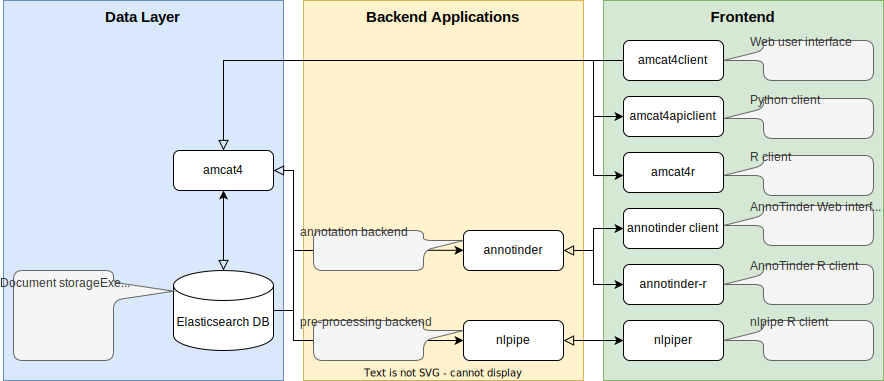
\includegraphics{media/amcat-flow.drawio.png}

}

\caption{amcat-framework}

\end{figure}%

It might seem like this is overly complicated, given that all of the
features are also available in other software packages, some of which
you will also be familiar with already. However, the main reason that
functions are split between different software modules is to make
development easier and more transparent. \textbf{If you are only
interested in amcat's capabilities, you can use it on
\hyperref[run-on-our-servers]{our servers} or conveniently install
everything at once through \hyperref[setup-through-docker]{docker}.}

If you want to learn more about the project, have a look at the
\hyperref[about-amcat]{about chapter}.

\bookmarksetup{startatroot}

\chapter{Getting started}\label{getting-started}

\begin{tcolorbox}[enhanced jigsaw, coltitle=black, breakable, title=\textcolor{quarto-callout-important-color}{\faExclamation}\hspace{0.5em}{Will change soon}, left=2mm, arc=.35mm, colback=white, colframe=quarto-callout-important-color-frame, toptitle=1mm, opacityback=0, bottomrule=.15mm, rightrule=.15mm, leftrule=.75mm, opacitybacktitle=0.6, bottomtitle=1mm, titlerule=0mm, toprule=.15mm, colbacktitle=quarto-callout-important-color!10!white]

\textbf{This is work in progress.} Passages highlighted in red are
likely to change soon.

\end{tcolorbox}

In this chapter, we show you how to download, set up, and start AmCAT.

\begin{figure}[H]

{\centering 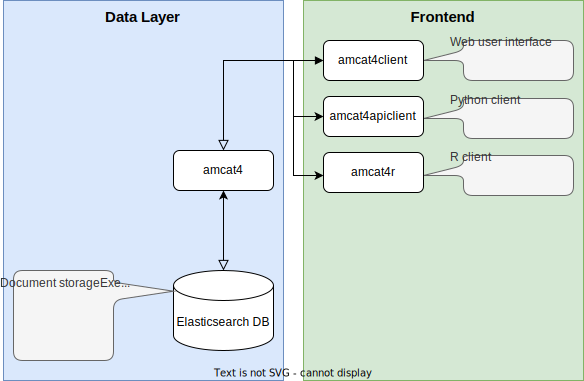
\includegraphics{media/amcat-flow-getting-started.drawio.png}

}

\caption{AmCAT instance after following this chapter}

\end{figure}%

In the \hyperref[Installing-and-accessing-AmCAT]{Installing and
accessing AmCAT} section, it is sufficient if you choose one of the
sub-sections to follow. We explain how you can run AmCAT

\begin{itemize}
\tightlist
\item
  \hyperref[run-on-our-servers]{on our servers}, which we recommend for
  testing purposes;
\item
  \hyperref[setup-through-docker]{through a Docker image}, which we
  recommend for most people who want to conduct a research project
  and/or share data online;
\item
  \hyperref[setup-on-your-own-server]{or install AmCAT directly on your
  system}, which we only recommend for advanced users, who want a
  customised setup.
\end{itemize}

In the \hyperref[frontend]{Frontend} section, it makes sense to cover
the \hyperref[amcat4client]{amcat4client}, which provides a react web
interface to query data. Then you can select to either install the
\hyperref[amcat4r]{R} or \hyperref[amcat4py]{Python} client.

\section{Installing and accessing
AmCAT}\label{installing-and-accessing-amcat}

\subsection{Run on our servers}\label{run-on-our-servers}

\begin{tcolorbox}[enhanced jigsaw, coltitle=black, breakable, title=\textcolor{quarto-callout-important-color}{\faExclamation}\hspace{0.5em}{Coming soon\ldots{}}, left=2mm, arc=.35mm, colback=white, colframe=quarto-callout-important-color-frame, toptitle=1mm, opacityback=0, bottomrule=.15mm, rightrule=.15mm, leftrule=.75mm, opacitybacktitle=0.6, bottomtitle=1mm, titlerule=0mm, toprule=.15mm, colbacktitle=quarto-callout-important-color!10!white]

\end{tcolorbox}

\subsection{AmCAT in your personal
computer}\label{amcat-in-your-personal-computer}

Let's first install AmCAT in your computer. For this, you need to:
1.Install Docker, 2.Copy the ``docker-compose.yml'' file in your
computer, and 3.Run the file via terminal. It sounds hard, but do not
worry, I will visually walk you through each step.

\subsubsection{Install Docker}\label{install-docker}

\begin{tcolorbox}[enhanced jigsaw, coltitle=black, breakable, title=\textcolor{quarto-callout-tip-color}{\faLightbulb}\hspace{0.5em}{Why do we use Docker for installation?}, left=2mm, arc=.35mm, colback=white, colframe=quarto-callout-tip-color-frame, toptitle=1mm, opacityback=0, bottomrule=.15mm, rightrule=.15mm, leftrule=.75mm, opacitybacktitle=0.6, bottomtitle=1mm, titlerule=0mm, toprule=.15mm, colbacktitle=quarto-callout-tip-color!10!white]

Functionally, Docker containers are a cross-platform installation format
that makes it trivially easy to install software packages on Linux,
MacOS and Windows without needing users to deal with dependency issues
or installation quirks on different systems.\footnotemark{} A side
effect is that we can easily develop AmCAT for all operating systems at
once and you can be sure that we do not fall behind on developing AmCAT
for your operating system of choice.

\end{tcolorbox}

\footnotetext{ Technically, it is a little more complicated, as Docker
containers have many similarities to virtual machines. However, for most
users that technical background is not really important. If you want to
learn more, have a look
\href{https://www.docker.com/resources/what-container/}{here}.}

Docker is a software that allows easy creation and portability of
software in something called containers. AmCAT is stored in one of such
containers. To install it, you need to first install Docker:
\url{https://www.docker.com/get-started/}. To install Docker, you can
head over to the Docker website to get
\href{https://docs.docker.com/get-docker/}{Docker Desktop} or the
\href{https://docs.docker.com/engine/install/}{Docker Engine} and
\href{https://docs.docker.com/compose/install/}{Docker Compose} to use
Docker from the command line.\footnote{On Ubuntu and Debian, the Docker
  Compose version in the repos is too old. You can use this gist to
  update it:
  \url{https://gist.github.com/JBGruber/db4de49ee106889b969a277f800c05b8}}
For a visual guide, you can check the video Johannes Gruber (2024) made:
\url{https://www.youtube.com/watch?v=iMyCdd5nP5U}. Remember that to use
Docker, you do NOT need to create an account.

Docker Desktop makes installation easier if you do not use a package
manager (which many Windows and MacOS users do not). Docker Desktop
looks like this:

\begin{figure}[H]

{\centering \includegraphics[width=6.25in,height=\textheight]{media/amcat-2.1.2_1.png}

}

\caption{Docker\_Desktop}

\end{figure}%

\subsubsection{Copy the docker-compose.yml file in your
computer}\label{copy-the-docker-compose.yml-file-in-your-computer}

To install the AmCAT data layer, you should use our Docker Compose file.
You can get it from
\href{https://raw.githubusercontent.com/ccs-amsterdam/amcat4docker/main/docker-compose.yml}{here}
(save the file as ``docker-compose.yml'').

In general, Gruber (2024) explains how to copy a ``docker-compose.yml''
file depending on the Operating System (OS). Here, we visually follow
the steps for the AmCAT ``docker-compose.yml'' using a Windows OS.
Access the AmCAT ``docker-compose.yml'' here:
\url{https://raw.githubusercontent.com/ccs-amsterdam/amcat4docker/main/docker-compose.yml}.

\begin{figure}[H]

{\centering \includegraphics[width=6.25in,height=\textheight]{media/amcat-2.1.2_2.png}

}

\caption{AmCAT\_DockerCompose1}

\end{figure}%

Now, press the right button of your mouse. That will display the
following menu:

\begin{figure}[H]

{\centering \includegraphics[width=6.25in,height=\textheight]{media/amcat-2.1.2_3.png}

}

\caption{AmCAT\_DockerCompose2}

\end{figure}%

From there, press the option ``Save Page As\ldots{}'' and save it in any
location you want:

\begin{figure}[H]

{\centering \includegraphics[width=6.25in,height=\textheight]{media/amcat-2.1.2_4.png}

}

\caption{AmCAT\_DockerCompose3}

\end{figure}%

By default, Windows saves any ``weird'' file as ``txt'':

\begin{figure}[H]

{\centering \includegraphics[width=6.25in,height=\textheight]{media/amcat-2.1.2_5.png}

}

\caption{AmCAT\_DockerCompose4}

\end{figure}%

So, we need to explicitly tell Windows that our file is a ``yml'' type.
To do so, you need to press View/Show/File name extensions:

\begin{figure}[H]

{\centering \includegraphics[width=6.25in,height=\textheight]{media/amcat-2.1.2_7.png}

}

\caption{AmCAT\_DockerCompose5}

\end{figure}%

Now, you can see that Windows added the ``txt'' extension to the file:

\begin{figure}[H]

{\centering \includegraphics[width=6.25in,height=\textheight]{media/amcat-2.1.2_8.png}

}

\caption{AmCAT\_DockerCompose6}

\end{figure}%

All we need to do is to delete the extra ``.txt'':

\begin{figure}[H]

{\centering \includegraphics[width=6.25in,height=\textheight]{media/amcat-2.1.2_9.png}

}

\caption{AmCAT\_DockerCompose7}

\end{figure}%

Now the file type changes to ``YML file''.

\subsubsection{Run the file via
terminal}\label{run-the-file-via-terminal}

Now, we will run the file via terminal. Gruber (2024)
\url{https://www.youtube.com/watch?v=iMyCdd5nP5U} shows how to do so
depending on the OS. Here, we will do it for Windows. So, let's open
``Windows PowerShell'':

\begin{figure}[H]

{\centering \includegraphics[width=6.25in,height=\textheight]{media/amcat-2.1.2_10.png}

}

\caption{Windows Power Shell}

\end{figure}%

This will open the following window:

\begin{figure}[H]

{\centering \includegraphics[width=6.25in,height=\textheight]{media/amcat-2.1.2_11.png}

}

\caption{Windows Power Shell}

\end{figure}%

In here, we will: (a) move to the folder where the
``docker-compose.yml'' is, and (b) run the ``docker-compose.yml'' file.

\textbf{(a) Move to the folder where the ``docker-compose.yml'' is}

For that, you will use the command \texttt{cd} followed by the path
where the file is. For example, mine is in the ``Download'' folder,
therefore, my command looks like:

\begin{figure}[H]

{\centering \includegraphics[width=6.25in,height=\textheight]{media/amcat-2.1.2_12.png}

}

\caption{Change Directory}

\end{figure}%

Now press enter. This will modify how the previous link looks like:

\begin{figure}[H]

{\centering \includegraphics[width=6.25in,height=\textheight]{media/amcat-2.1.2_13.png}

}

\caption{Change Directory2}

\end{figure}%

\textbf{(b) Run the ``docker-compose.yml'' file}

Now, you need to run the following command:

\texttt{\#\ docker-compose\ up\ -\/-pull="missing"\ -d}

\begin{figure}[H]

{\centering \includegraphics[width=6.25in,height=\textheight]{media/amcat-2.1.2_14.png}

}

\caption{Docker compose}

\end{figure}%

Once it finishes running, it will show the following:

\begin{figure}[H]

{\centering \includegraphics[width=6.25in,height=\textheight]{media/amcat-2.1.2_15.png}

}

\caption{Docker compose2}

\end{figure}%

If you navigate to Docker Desktop, you will see that AmCAT, together
with other dependencies, is now listed as a container under
``downloads'':

\begin{figure}[H]

{\centering \includegraphics[width=6.25in,height=\textheight]{media/amcat-2.1.2_16.png}

}

\caption{Docker Desktop with AmCAT}

\end{figure}%

We tried to write the file to contain sensible defaults for testing it
locally. If you plan to work with AmCAT for a research project and/or
plan to update the images in the future, you should have a look at the
customization option. Otherwise, you can continue.

\begin{tcolorbox}[enhanced jigsaw, coltitle=black, breakable, title=\textcolor{quarto-callout-note-color}{\faInfo}\hspace{0.5em}{Customization}, left=2mm, arc=.35mm, colback=white, colframe=quarto-callout-note-color-frame, toptitle=1mm, opacityback=0, bottomrule=.15mm, rightrule=.15mm, leftrule=.75mm, opacitybacktitle=0.6, bottomtitle=1mm, titlerule=0mm, toprule=.15mm, colbacktitle=quarto-callout-note-color!10!white]

The current default docker-compose.yml looks like this:

\begin{Shaded}
\begin{Highlighting}[]
\NormalTok{docker\_compose }\OtherTok{\textless{}{-}} \FunctionTok{readLines}\NormalTok{(}\StringTok{"https://raw.githubusercontent.com/ccs{-}amsterdam/amcat4docker/main/docker{-}compose.yml"}\NormalTok{)}
\NormalTok{knitr}\SpecialCharTok{::}\FunctionTok{asis\_output}\NormalTok{(}\FunctionTok{paste0}\NormalTok{(}
  \StringTok{"\textasciigrave{}\textasciigrave{}\textasciigrave{} \{.bash code{-}line{-}numbers=}\SpecialCharTok{\textbackslash{}"}\StringTok{true}\SpecialCharTok{\textbackslash{}"}\StringTok{\}}\SpecialCharTok{\textbackslash{}n}\StringTok{"}\NormalTok{,}
  \FunctionTok{paste0}\NormalTok{(}
\NormalTok{    docker\_compose,}
    \AttributeTok{collapse =} \StringTok{"}\SpecialCharTok{\textbackslash{}n}\StringTok{"}
\NormalTok{  ),}
  \StringTok{"}\SpecialCharTok{\textbackslash{}n}\StringTok{\textasciigrave{}\textasciigrave{}\textasciigrave{}"}  
\NormalTok{))}
\end{Highlighting}
\end{Shaded}

\begin{Shaded}
\begin{Highlighting}[numbers=left,,]
\ExtensionTok{services:}
  \ExtensionTok{web\_server:}
    \ExtensionTok{image:}\NormalTok{ ccsamsterdam/ngincat:4.0.16}
    \ExtensionTok{build:}\NormalTok{ ./ngincat}
    \ExtensionTok{container\_name:}\NormalTok{ ngincat}
    \ExtensionTok{restart:}\NormalTok{ unless{-}stopped}
    \ExtensionTok{networks:}
      \ExtensionTok{{-}}\NormalTok{ amcat{-}net}
    \ExtensionTok{environment:}
      \ExtensionTok{{-}}\NormalTok{ amcat4\_client=}\VariableTok{$\{AMCAT\_CLIENT}\OperatorTok{:{-}}\NormalTok{http://amcat4client:3000}\VariableTok{\}}
      \ExtensionTok{{-}}\NormalTok{ amcat4\_host=}\VariableTok{$\{AMCAT\_HOST\_INTERNAL}\OperatorTok{:{-}}\NormalTok{http://amcat4:5000}\VariableTok{\}}
    \ExtensionTok{ports:}
      \ExtensionTok{{-}}\NormalTok{ 80:80 }\CommentTok{\# [local port]:[container port]}
    \ExtensionTok{depends\_on:}
      \ExtensionTok{{-}} \StringTok{"web\_client"}
      \ExtensionTok{{-}} \StringTok{"api"}
  \ExtensionTok{web\_client:}
    \ExtensionTok{image:}\NormalTok{ ccsamsterdam/amcat4client:4.0.16}
    \ExtensionTok{build:}\NormalTok{ ./amcat4client}
    \ExtensionTok{container\_name:}\NormalTok{ amcat4client}
    \ExtensionTok{restart:}\NormalTok{ unless{-}stopped}
    \ExtensionTok{networks:}
      \ExtensionTok{{-}}\NormalTok{ amcat{-}net}
    \ExtensionTok{environment:}
      \ExtensionTok{{-}}\NormalTok{ AMCAT\_SERVER=}\VariableTok{$\{AMCAT\_HOST\_EXTERNAL}\OperatorTok{:{-}}\NormalTok{http://localhost/amcat}\VariableTok{\}}
    \ExtensionTok{depends\_on:}
      \ExtensionTok{{-}} \StringTok{"api"}
  \ExtensionTok{api:}
    \ExtensionTok{image:}\NormalTok{ ccsamsterdam/amcat4:4.0.16}
    \ExtensionTok{build:}\NormalTok{ ./amcat4}
    \ExtensionTok{container\_name:}\NormalTok{ amcat4}
    \ExtensionTok{restart:}\NormalTok{ unless{-}stopped}
    \ExtensionTok{networks:}
      \ExtensionTok{{-}}\NormalTok{ amcat{-}net}
    \ExtensionTok{environment:}
      \CommentTok{\# note that these take precedence over values set in \textasciigrave{}amcat4 config\textasciigrave{}\textasciigrave{}}
      \ExtensionTok{{-}}\NormalTok{ amcat4\_elastic\_host=}\VariableTok{$\{ELASTIC\_HOST}\OperatorTok{:{-}}\NormalTok{http://elastic8:9200}\VariableTok{\}}
      \ExtensionTok{{-}}\NormalTok{ amcat4\_host=}\VariableTok{$\{AMCAT\_HOST\_EXTERNAL}\OperatorTok{:{-}}\NormalTok{http://localhost/amcat}\VariableTok{\}}
      \ExtensionTok{{-}}\NormalTok{ FORWARDED\_ALLOW\_IPS=}\PreprocessorTok{*}
    \ExtensionTok{depends\_on:}
      \ExtensionTok{{-}} \StringTok{"db"}
  \ExtensionTok{db:}
    \ExtensionTok{image:}\NormalTok{ docker.elastic.co/elasticsearch/elasticsearch:8.18.4}
    \ExtensionTok{container\_name:}\NormalTok{ elastic8}
    \ExtensionTok{restart:}\NormalTok{ unless{-}stopped}
    \CommentTok{\# for security reasons, the database is only exposed to the other containers in the amcat{-}net network}
    \CommentTok{\# If you want to be able to access it locally, uncomment the following two lines}
    \CommentTok{\# ports:}
    \CommentTok{\# {-} 9200:9200}
    \ExtensionTok{networks:}
      \ExtensionTok{{-}}\NormalTok{ amcat{-}net}
    \ExtensionTok{environment:}
      \ExtensionTok{{-}}\NormalTok{ discovery.type=single{-}node}
      \ExtensionTok{{-}}\NormalTok{ bootstrap.memory\_lock=true}
      \CommentTok{\# limits memory usage of elasticsearch; 4g or less can cause errors when uploading larger document collections}
      \ExtensionTok{{-}} \StringTok{"ES\_JAVA\_OPTS={-}Xms4g {-}Xmx4g"}
      \ExtensionTok{{-}}\NormalTok{ xpack.security.enabled=false}
    \CommentTok{\# your database should have a folder on the host machine to permanently store data. By default}
    \CommentTok{\# a docker volume (called elastic{-}volume) is used, which leaves management of the files to Docker}
    \CommentTok{\# (see https://docs.docker.com/storage/volumes/). You can also store files somewhere else with}
    \CommentTok{\# (for example):}
    \CommentTok{\#}
    \CommentTok{\# volumes:}
    \CommentTok{\#   {-} /path/to/elastic{-}data:/usr/share/elasticsearch/data \# [local path]:[container path]}
    \CommentTok{\#}
    \CommentTok{\# In this case, you need to make sure that the folder \textasciigrave{}/path/to/elastic{-}data\textasciigrave{} exists and Docker}
    \CommentTok{\# has read and write access to it.}
    \ExtensionTok{volumes:}
      \ExtensionTok{{-}}\NormalTok{ elastic{-}volume:/usr/share/elasticsearch/data:rw}

\ExtensionTok{networks:}
  \ExtensionTok{amcat{-}net:}

\ExtensionTok{volumes:}
     \ExtensionTok{elastic{-}volume:}
\end{Highlighting}
\end{Shaded}

Setting the containers up from \texttt{R} or \texttt{Python} uses the
same settings. You can leave most lines as they are, but we want to draw
your attention to a couple of settings you might want to change:

\begin{itemize}
\tightlist
\item
  In lines 12, 13, we set the port to \texttt{80} on the host machine.
  This means you will be able to access the AmCAT client without
  specifying a port (80 is the default port your browser uses to access
  an address). If the port is already in use, the container will crash.
  In this case, change \texttt{80}to a different port and access AmCAT
  through, for example, \texttt{localhost:5000}.
\item
  In lines 53, 54, 55, 56, we configured Elasticsearch to form a
  single-node cluster and use a maximum of 4GB memory.
\item
  In lines 63, 64 we suggested a setting so Elasticsearch will store
  your data on a volume on the host machine. \textbf{If you do not use
  this, your data will be destroyed when you remove the Elasticsearch
  container!}. We recommend this to make it easier to back up your
  database and reuse it with a different installation of Elasticsearch
  (e.g., after an update) in the future. However, the container will not
  run if it does not have proper access to this folder. See the comment
  to solve this. Note that the suggested local path is just an example.
  Learn more about this in the chapter
  \hyperref[backupux2c-restore-and-update-amcat]{on backups and
  updates}.
\end{itemize}

\end{tcolorbox}

\bookmarksetup{startatroot}

\chapter{Document Storage}\label{document-storage}

This chapter covers how you can upload, change, query, and delete
documents and indexes in AmCAT. Some basic tasks are implemented in the
\hyperref[manage-documents-with-a-client]{Web user interface}, for the
rest you need to use \hyperref[manage-documents-with-a-client]{one of
the clients} in \texttt{R} or \texttt{Python} or another means to call
the API (e.g., through \href{https://en.wikipedia.org/wiki/CURL}{cURL}
as shown below). You can also use the API calls to build your own
client.

More information on the API can be found on every amcat4 instance at
\texttt{/redoc} (e.g., \url{http://localhost/amcat/redoc}).

Let us know about it and we will promote your new API wrapper package
here.

\section{Manage Documents with the Graphic User
Interface}\label{manage-documents-with-the-graphic-user-interface}

\subsection{Upload}\label{upload}

From the Graphic User Interface (GUI), you can ``Create an Index'' by
uploading it as a csv file.

Navigate to your favorite spreadsheet (e.g.~Excel) and create something
that resembles the following:

\includegraphics{media/amcat-3.1-1.png}

Save it as csv utf-8:

\includegraphics{media/amcat-3.1-2.png}

Upload it to AmCAT:

\includegraphics{media/amcat-3.1-3.png}

Fill out each option and press ``Create'':

\includegraphics{media/amcat-3.1-4.png}

That will display a window with the following information:

\includegraphics{media/amcat-3.1-5.png}

Now, you can just drag and drop the csv file into the window:

\includegraphics{media/amcat-3.1-6.png}

This will display a window with the following information:

\includegraphics{media/amcat-3.1-7.png}

From there, you can either choose the type of field by clicking ``Select
field'' or let AmCAT do it for you by clicking ``automate''. If in
doubt, then choose ``automate''. Clicking ``automate'' on all gives the
following result:

\includegraphics{media/amcat-3.1-8.png}

You have to explicitly choose the column(s) that will be used to create
the unique identifier. In this example, I explicitly created a column
named ``id''. So, that is the one I chose as identifier:

\includegraphics{media/amcat-3.1-9.png}

Now, you can press ``Upload 15 documents'', which is the number of rows
in the csv file.

\includegraphics{media/amcat-3.1-10.png}

Now you can navigate to your indeces and find your newly made index:

\includegraphics{media/amcat-3.1-11.png}

\subsection{Visualize}\label{visualize}

One of AmCAT features is that it allows you to perform some basic
visualizations. To do so in the main window, you first need to enable
them.

For this, you just need to click on ``Enable visualizations in field
settings''.

\includegraphics{media/amcat-3.2-1.png}

That will open the following window:

\includegraphics{media/amcat-3.2-2.png}

From there, you just need to click on the fields
\includegraphics{media/amcat-3.2-3.png}, under the column ``Display'',
and choose the options ``show as heading'' and/or ``visualize in list''.

\includegraphics{media/amcat-3.2-4.png}

You can go back to the main window by clicking on ``Dashboard''
\includegraphics{media/amcat-3.2-5.png}. There you can see the
visualizations you have enabled:

\includegraphics{media/amcat-3.2-6.png}

\section{Manage Documents with the
API}\label{manage-documents-with-the-api}

For this overview, we log into a local \texttt{amcat4} (i.e.,
\texttt{http://localhost/amcat}). Replace this with the address to the
\texttt{amcat4} instance you are working with (e.g.,
\texttt{https://opted.amcat.nl/api}).

We first need to log in:

\subsubsection{R}

\begin{Shaded}
\begin{Highlighting}[]
\FunctionTok{library}\NormalTok{(amcat4r)}
\FunctionTok{amcat\_login}\NormalTok{(}\StringTok{"http://localhost/amcat"}\NormalTok{)}
\end{Highlighting}
\end{Shaded}

\subsubsection{Python}

\begin{Shaded}
\begin{Highlighting}[]
\ImportTok{from}\NormalTok{ amcat4py }\ImportTok{import}\NormalTok{ AmcatClient}
\NormalTok{amcat }\OperatorTok{=}\NormalTok{ AmcatClient(}\StringTok{"http://localhost/amcat"}\NormalTok{)}
\ControlFlowTok{if}\NormalTok{ amcat.login\_required():}
\NormalTok{    amcat.login()}
\end{Highlighting}
\end{Shaded}

\subsubsection{cURL}

There is no dedicated way at the moment to get a token via cURL. You can
still use cURL with instances that do not require authentication or by
copying the token from \texttt{Python} or \texttt{R}. In these cases,
you can make requests with an extra header, for example:

\begin{Shaded}
\begin{Highlighting}[]
\VariableTok{AMCAT\_TOKEN}\OperatorTok{=}\StringTok{"YOUR\_TOKEN"}
\ExtensionTok{curl} \AttributeTok{{-}s}\NormalTok{ http://localhost/amcat/index/ }\DataTypeTok{\textbackslash{}}
  \AttributeTok{{-}H} \StringTok{"Authorization: Bearer }\VariableTok{$\{AMCAT\_TOKEN\}}\StringTok{"}
\end{Highlighting}
\end{Shaded}

We can first list all available indexes, as a document collection is
called in Elasticsearch and thus in AmCAT:

\subsubsection{R}

\begin{Shaded}
\begin{Highlighting}[]
\FunctionTok{list\_indexes}\NormalTok{()}
\end{Highlighting}
\end{Shaded}

\subsubsection{Python}

\begin{Shaded}
\begin{Highlighting}[]
\NormalTok{amcat.list\_indices()}
\end{Highlighting}
\end{Shaded}

\subsubsection{cURL}

\begin{Shaded}
\begin{Highlighting}[]
\ExtensionTok{curl} \AttributeTok{{-}s}\NormalTok{ http://localhost/amcat/index/}
\end{Highlighting}
\end{Shaded}

You can see that the test index we added in the
\hyperref[data-layer]{Data Layer} section is here and that it is called
``state\_of\_the\_union''. To see everyone who has been granted access
to an index we can use:

\subsubsection{R}

\begin{Shaded}
\begin{Highlighting}[]
\FunctionTok{list\_index\_users}\NormalTok{(}\AttributeTok{index =} \StringTok{"state\_of\_the\_union"}\NormalTok{)}
\end{Highlighting}
\end{Shaded}

\subsubsection{Python}

\begin{Shaded}
\begin{Highlighting}[]
\NormalTok{amcat.list\_index\_users(index}\OperatorTok{=}\StringTok{"state\_of\_the\_union"}\NormalTok{)}
\end{Highlighting}
\end{Shaded}

\subsubsection{cURL}

\begin{Shaded}
\begin{Highlighting}[]
\ExtensionTok{curl} \AttributeTok{{-}s}\NormalTok{ http://localhost/amcat/index/state\_of\_the\_union/users}
\end{Highlighting}
\end{Shaded}

We will learn more about these roles in the chapter on
\hyperref[document-sharing-and-access-management]{access management}. To
see what an index looks like, we can query it leaving all fields blank
to request all data at once:

\subsubsection{R}

\begin{Shaded}
\begin{Highlighting}[]
\NormalTok{sotu }\OtherTok{\textless{}{-}} \FunctionTok{query\_documents}\NormalTok{(}\AttributeTok{index =} \StringTok{"state\_of\_the\_union"}\NormalTok{, }\AttributeTok{queries =} \ConstantTok{NULL}\NormalTok{, }\AttributeTok{fields =} \ConstantTok{NULL}\NormalTok{)}
\FunctionTok{str}\NormalTok{(sotu)}
\end{Highlighting}
\end{Shaded}

\subsubsection{Python}

\begin{Shaded}
\begin{Highlighting}[]
\NormalTok{sotu }\OperatorTok{=} \BuiltInTok{list}\NormalTok{(amcat.query(}\StringTok{"state\_of\_the\_union"}\NormalTok{, fields}\OperatorTok{=}\VariableTok{None}\NormalTok{))}
\BuiltInTok{print}\NormalTok{(}\BuiltInTok{len}\NormalTok{(sotu))}
\ControlFlowTok{for}\NormalTok{ k, v }\KeywordTok{in}\NormalTok{ sotu[}\DecValTok{1}\NormalTok{].items():}
  \BuiltInTok{print}\NormalTok{(k }\OperatorTok{+} \StringTok{"("} \OperatorTok{+} \BuiltInTok{str}\NormalTok{(}\BuiltInTok{type}\NormalTok{(v)) }\OperatorTok{+} \StringTok{"): "} \OperatorTok{+} \BuiltInTok{str}\NormalTok{(v)[}\DecValTok{0}\NormalTok{:}\DecValTok{100}\NormalTok{] }\OperatorTok{+} \StringTok{"..."}\NormalTok{)}
\end{Highlighting}
\end{Shaded}

\subsubsection{cURL}

To not clog the output, we save it into file and display only the
beginning:

\begin{Shaded}
\begin{Highlighting}[]
\ExtensionTok{curl} \AttributeTok{{-}s}\NormalTok{ http://localhost/amcat/index/state\_of\_the\_union/documents }\OperatorTok{\textgreater{}}\NormalTok{ sotu.json}
\CommentTok{\# show the first few characters only}
\FunctionTok{head} \AttributeTok{{-}c}\NormalTok{ 150 sotu.json}
\end{Highlighting}
\end{Shaded}

Knowing now what a document should look like in this index, we can
upload a new document to get familiar with the process:

\subsubsection{R}

\begin{Shaded}
\begin{Highlighting}[]
\NormalTok{new\_doc }\OtherTok{\textless{}{-}} \FunctionTok{data.frame}\NormalTok{(}
  \AttributeTok{title =} \StringTok{"test"}\NormalTok{,}
  \AttributeTok{text =} \StringTok{"test"}\NormalTok{,}
  \AttributeTok{date =} \FunctionTok{as.Date}\NormalTok{(}\StringTok{"2022{-}01{-}01"}\NormalTok{),}
  \AttributeTok{president =} \StringTok{"test"}\NormalTok{,}
  \AttributeTok{year =} \StringTok{"2022"}\NormalTok{,}
  \AttributeTok{party =} \StringTok{"test"}\NormalTok{,}
  \AttributeTok{url =} \StringTok{"test"}
\NormalTok{)}
\FunctionTok{upload\_documents}\NormalTok{(}\AttributeTok{index =} \StringTok{"state\_of\_the\_union"}\NormalTok{, new\_doc)}
\end{Highlighting}
\end{Shaded}

\subsubsection{Python}

\begin{Shaded}
\begin{Highlighting}[]
\ImportTok{from}\NormalTok{ datetime }\ImportTok{import}\NormalTok{ datetime}
\NormalTok{new\_doc }\OperatorTok{=}\NormalTok{ \{}
  \StringTok{"title"}\NormalTok{: }\StringTok{"test"}\NormalTok{,}
  \StringTok{"text"}\NormalTok{: }\StringTok{"test"}\NormalTok{,}
  \StringTok{"date"}\NormalTok{: datetime.strptime(}\StringTok{"2022{-}01{-}01"}\NormalTok{, }\StringTok{\textquotesingle{}\%Y{-}\%m{-}}\SpecialCharTok{\%d}\StringTok{\textquotesingle{}}\NormalTok{),}
  \StringTok{"president"}\NormalTok{: }\StringTok{"test"}\NormalTok{,}
  \StringTok{"year"}\NormalTok{: }\StringTok{"2022"}\NormalTok{,}
  \StringTok{"party"}\NormalTok{: }\StringTok{"test"}\NormalTok{,}
  \StringTok{"url"}\NormalTok{: }\StringTok{"test"}
\NormalTok{\}}
\NormalTok{amcat.upload\_documents(}\StringTok{"state\_of\_the\_union"}\NormalTok{, [new\_doc])}
\end{Highlighting}
\end{Shaded}

\subsubsection{cURL}

\begin{Shaded}
\begin{Highlighting}[]
\ExtensionTok{curl} \AttributeTok{{-}s} \AttributeTok{{-}X}\NormalTok{ POST http://localhost/amcat/index/state\_of\_the\_union/documents }\DataTypeTok{\textbackslash{}}
  \AttributeTok{{-}H} \StringTok{"Content{-}Type: application/json"} \DataTypeTok{\textbackslash{}}
  \AttributeTok{{-}d} \StringTok{\textquotesingle{}\{}
\StringTok{         "documents":[}
\StringTok{            \{}
\StringTok{               "title":"test",}
\StringTok{               "text":"test",}
\StringTok{               "date":"2022{-}01{-}01",}
\StringTok{               "president":"test",}
\StringTok{               "year":"2022",}
\StringTok{               "party":"test",}
\StringTok{               "url":"test"}
\StringTok{            \}}
\StringTok{         ]}
\StringTok{      \}\textquotesingle{}}
\end{Highlighting}
\end{Shaded}

Let's see if the the new document is in the index:

\subsubsection{R}

\begin{Shaded}
\begin{Highlighting}[]
\FunctionTok{query\_documents}\NormalTok{(}\AttributeTok{index =} \StringTok{"state\_of\_the\_union"}\NormalTok{, }\AttributeTok{fields =} \ConstantTok{NULL}\NormalTok{, }\AttributeTok{filters =} \FunctionTok{list}\NormalTok{(}\AttributeTok{title =} \StringTok{"test"}\NormalTok{))}
\end{Highlighting}
\end{Shaded}

\subsubsection{Python}

\begin{Shaded}
\begin{Highlighting}[]
\ImportTok{import}\NormalTok{ pprint}
\NormalTok{pp }\OperatorTok{=}\NormalTok{ pprint.PrettyPrinter(depth}\OperatorTok{=}\DecValTok{4}\NormalTok{)}
\NormalTok{res}\OperatorTok{=}\BuiltInTok{list}\NormalTok{(amcat.query(}\StringTok{"state\_of\_the\_union"}\NormalTok{, fields}\OperatorTok{=}\VariableTok{None}\NormalTok{, filters}\OperatorTok{=}\NormalTok{\{}\StringTok{"title"}\NormalTok{: }\StringTok{"test"}\NormalTok{\}))}
\NormalTok{pp.pprint(res)}
\end{Highlighting}
\end{Shaded}

\subsubsection{cURL}

\begin{Shaded}
\begin{Highlighting}[]
\ExtensionTok{curl} \AttributeTok{{-}s} \AttributeTok{{-}X}\NormalTok{ POST http://localhost/amcat/index/state\_of\_the\_union/query }\DataTypeTok{\textbackslash{}}
  \AttributeTok{{-}H} \StringTok{\textquotesingle{}Content{-}Type: application/json\textquotesingle{}} \DataTypeTok{\textbackslash{}}
  \AttributeTok{{-}d} \StringTok{\textquotesingle{}\{"filters":\{"title":["test"]\}\}\textquotesingle{}} \KeywordTok{|} \ExtensionTok{jq} \AttributeTok{{-}r} \StringTok{".results"}
\end{Highlighting}
\end{Shaded}

We will learn more about queries later on in the \href{}{Writing a
Query} chapter.

Instead of adding whole documents, you can also change fields in an
index. Fields are similar to columns in a table in Excel. However, you
need to define the type of a field upon its creation and make sure that
you later only add data which adheres to the specifications of the type
(otherwise you will get an error). To learn more about the fields in the
test index, you can use:

\subsubsection{R}

\begin{Shaded}
\begin{Highlighting}[]
\FunctionTok{get\_fields}\NormalTok{(}\AttributeTok{index =} \StringTok{"state\_of\_the\_union"}\NormalTok{)}
\end{Highlighting}
\end{Shaded}

\subsubsection{Python}

\begin{Shaded}
\begin{Highlighting}[]
\NormalTok{amcat.get\_fields(}\StringTok{"state\_of\_the\_union"}\NormalTok{)}
\end{Highlighting}
\end{Shaded}

\subsubsection{cURL}

\begin{Shaded}
\begin{Highlighting}[]
\ExtensionTok{curl} \AttributeTok{{-}s}\NormalTok{ http://localhost/amcat/index/state\_of\_the\_union/fields}
\end{Highlighting}
\end{Shaded}

You can see that there are five different types in this index: date,
keyword, text, url and double. Keyword, text, url are all essentially
the same type in \texttt{R}, namely character strings. The date needs to
be a \texttt{POSIXct} class, which you can create with \texttt{as.Date}.
Year should be a double, i.e., a numeric value or integer.

You can add new fields to this, for example, if you want to add a
keyword to the documents:

\subsubsection{R}

\begin{Shaded}
\begin{Highlighting}[]
\FunctionTok{set\_fields}\NormalTok{(}\AttributeTok{index =} \StringTok{"state\_of\_the\_union"}\NormalTok{, }\FunctionTok{list}\NormalTok{(}\AttributeTok{keyword =} \StringTok{"keyword"}\NormalTok{))}
\end{Highlighting}
\end{Shaded}

\subsubsection{Python}

\begin{Shaded}
\begin{Highlighting}[]
\NormalTok{amcat.set\_fields(}\StringTok{"state\_of\_the\_union"}\NormalTok{, \{}\StringTok{"keyword"}\NormalTok{:}\StringTok{"keyword"}\NormalTok{\})}
\end{Highlighting}
\end{Shaded}

\subsubsection{cURL}

\begin{Shaded}
\begin{Highlighting}[]
\ExtensionTok{curl} \AttributeTok{{-}s} \AttributeTok{{-}X}\NormalTok{ POST http://localhost/amcat/index/state\_of\_the\_union/fields }\DataTypeTok{\textbackslash{}}
  \AttributeTok{{-}H} \StringTok{\textquotesingle{}Content{-}Type: application/json\textquotesingle{}} \DataTypeTok{\textbackslash{}}
  \AttributeTok{{-}d} \StringTok{\textquotesingle{}\{"keyword":"keyword"\}\textquotesingle{}}
\end{Highlighting}
\end{Shaded}

When you now query a document, however, you will not see this new field:

\subsubsection{R}

\begin{Shaded}
\begin{Highlighting}[]
\FunctionTok{query\_documents}\NormalTok{(}\AttributeTok{index =} \StringTok{"state\_of\_the\_union"}\NormalTok{, }\AttributeTok{fields =} \ConstantTok{NULL}\NormalTok{, }\AttributeTok{filters =} \FunctionTok{list}\NormalTok{(}\AttributeTok{title =} \StringTok{"test"}\NormalTok{))}
\end{Highlighting}
\end{Shaded}

\subsubsection{Python}

\begin{Shaded}
\begin{Highlighting}[]
\NormalTok{res }\OperatorTok{=} \BuiltInTok{list}\NormalTok{(amcat.query(}\StringTok{"state\_of\_the\_union"}\NormalTok{, fields}\OperatorTok{=}\VariableTok{None}\NormalTok{, filters}\OperatorTok{=}\NormalTok{\{}\StringTok{"title"}\NormalTok{: }\StringTok{"test"}\NormalTok{\}))}
\NormalTok{pp.pprint(res)}
\end{Highlighting}
\end{Shaded}

\subsubsection{cURL}

\begin{Shaded}
\begin{Highlighting}[]
\ExtensionTok{curl} \AttributeTok{{-}s} \AttributeTok{{-}X}\NormalTok{ POST http://localhost/amcat/index/state\_of\_the\_union/query }\DataTypeTok{\textbackslash{}}
  \AttributeTok{{-}H} \StringTok{\textquotesingle{}Content{-}Type: application/json\textquotesingle{}} \DataTypeTok{\textbackslash{}}
  \AttributeTok{{-}d} \StringTok{\textquotesingle{}\{"filters":\{"title":["test"]\}\}\textquotesingle{}} \KeywordTok{|} \ExtensionTok{jq} \AttributeTok{{-}r} \StringTok{".results"}
\end{Highlighting}
\end{Shaded}

This is because it is empty for this document, just as the url field,
which is absent from all documents in this index. We can add something
to the new field and see if it shows up:

\subsubsection{R}

\begin{Shaded}
\begin{Highlighting}[]
\FunctionTok{update\_tags}\NormalTok{(}\AttributeTok{index =} \StringTok{"state\_of\_the\_union"}\NormalTok{, }
            \AttributeTok{action =} \StringTok{"add"}\NormalTok{, }
            \AttributeTok{field =} \StringTok{"keyword"}\NormalTok{, }
            \AttributeTok{tag =} \StringTok{"test"}\NormalTok{, }
            \AttributeTok{filters =} \FunctionTok{list}\NormalTok{(}\AttributeTok{title =} \StringTok{"test"}\NormalTok{))}
\end{Highlighting}
\end{Shaded}

\begin{Shaded}
\begin{Highlighting}[]
\FunctionTok{query\_documents}\NormalTok{(}\AttributeTok{index =} \StringTok{"state\_of\_the\_union"}\NormalTok{, }
                \AttributeTok{fields =} \FunctionTok{c}\NormalTok{(}\StringTok{"title"}\NormalTok{, }\StringTok{"keyword"}\NormalTok{),}
                \AttributeTok{filters =} \FunctionTok{list}\NormalTok{(}\AttributeTok{title =} \StringTok{"test"}\NormalTok{))}
\end{Highlighting}
\end{Shaded}

\subsubsection{Python}

\begin{Shaded}
\begin{Highlighting}[]
\NormalTok{test\_doc }\OperatorTok{=} \BuiltInTok{list}\NormalTok{(amcat.query(}\StringTok{"state\_of\_the\_union"}\NormalTok{, fields}\OperatorTok{=}\NormalTok{[}\StringTok{"id"}\NormalTok{], filters}\OperatorTok{=}\NormalTok{\{}\StringTok{"title"}\NormalTok{: }\StringTok{"test"}\NormalTok{\}))[}\DecValTok{0}\NormalTok{]}
\NormalTok{amcat.update\_document(}\StringTok{"state\_of\_the\_union"}\NormalTok{, doc\_id}\OperatorTok{=}\NormalTok{test\_doc[}\StringTok{"\_id"}\NormalTok{], body}\OperatorTok{=}\NormalTok{\{}\StringTok{"keyword"}\NormalTok{: }\StringTok{"test"}\NormalTok{\})}
\end{Highlighting}
\end{Shaded}

\begin{Shaded}
\begin{Highlighting}[]
\NormalTok{res}\OperatorTok{=}\BuiltInTok{list}\NormalTok{(amcat.query(}\StringTok{"state\_of\_the\_union"}\NormalTok{, fields}\OperatorTok{=}\NormalTok{[}\StringTok{"title"}\NormalTok{, }\StringTok{"keyword"}\NormalTok{], filters}\OperatorTok{=}\NormalTok{\{}\StringTok{"title"}\NormalTok{: }\StringTok{"test"}\NormalTok{\}))}
\NormalTok{pp.pprint(res)}
\end{Highlighting}
\end{Shaded}

\subsubsection{cURL}

\begin{Shaded}
\begin{Highlighting}[]
\VariableTok{test\_doc}\OperatorTok{=}\VariableTok{$(}\ExtensionTok{curl} \AttributeTok{{-}s} \AttributeTok{{-}X}\NormalTok{ POST http://localhost/amcat/index/state\_of\_the\_union/query }\DataTypeTok{\textbackslash{}}
  \AttributeTok{{-}H} \StringTok{\textquotesingle{}Content{-}Type: application/json\textquotesingle{}} \DataTypeTok{\textbackslash{}}
  \AttributeTok{{-}d} \StringTok{\textquotesingle{}\{"filters":\{"title":["test"]\}\}\textquotesingle{}} \KeywordTok{|} \ExtensionTok{jq} \AttributeTok{{-}r} \StringTok{".results[].\_id"}\VariableTok{)}
\ExtensionTok{curl} \AttributeTok{{-}s} \AttributeTok{{-}X}\NormalTok{ PUT http://localhost/amcat/index/state\_of\_the\_union/documents/}\VariableTok{$\{test\_doc\}} \DataTypeTok{\textbackslash{}}
  \AttributeTok{{-}H} \StringTok{\textquotesingle{}Content{-}Type: application/json\textquotesingle{}} \DataTypeTok{\textbackslash{}}
  \AttributeTok{{-}d} \StringTok{\textquotesingle{}\{"keyword": "test"\}\textquotesingle{}}
\end{Highlighting}
\end{Shaded}

\begin{Shaded}
\begin{Highlighting}[]
\ExtensionTok{curl} \AttributeTok{{-}s} \AttributeTok{{-}X}\NormalTok{ POST http://localhost/amcat/index/state\_of\_the\_union/query }\DataTypeTok{\textbackslash{}}
  \AttributeTok{{-}H} \StringTok{\textquotesingle{}Content{-}Type: application/json\textquotesingle{}} \DataTypeTok{\textbackslash{}}
  \AttributeTok{{-}d} \StringTok{\textquotesingle{}\{"filters":\{"title":["test"]\}\}\textquotesingle{}} \KeywordTok{|} \ExtensionTok{jq} \AttributeTok{{-}r} \StringTok{".results"}
\end{Highlighting}
\end{Shaded}

Now that we have a better idea of what an index is and how it looks
like, we can create a new one\textgreater{}

\subsubsection{R}

\begin{Shaded}
\begin{Highlighting}[]
\FunctionTok{create\_index}\NormalTok{(}\AttributeTok{index =} \StringTok{"new\_index"}\NormalTok{, }\AttributeTok{guest\_role =} \StringTok{"admin"}\NormalTok{)}
\FunctionTok{list\_indexes}\NormalTok{()}
\FunctionTok{get\_fields}\NormalTok{(}\AttributeTok{index =} \StringTok{"new\_index"}\NormalTok{)}
\end{Highlighting}
\end{Shaded}

\subsubsection{Python}

\begin{Shaded}
\begin{Highlighting}[]
\NormalTok{amcat.create\_index(index}\OperatorTok{=}\StringTok{"new\_index"}\NormalTok{, guest\_role}\OperatorTok{=}\StringTok{"admin"}\NormalTok{)}
\end{Highlighting}
\end{Shaded}

\begin{Shaded}
\begin{Highlighting}[]
\NormalTok{amcat.list\_indices()}
\NormalTok{amcat.get\_fields(}\StringTok{"new\_index"}\NormalTok{)}
\end{Highlighting}
\end{Shaded}

\subsubsection{cURL}

\begin{Shaded}
\begin{Highlighting}[]
\ExtensionTok{curl} \AttributeTok{{-}s} \AttributeTok{{-}X}\NormalTok{ POST http://localhost/amcat/index/ }\DataTypeTok{\textbackslash{}}
  \AttributeTok{{-}H} \StringTok{\textquotesingle{}Content{-}Type: application/json\textquotesingle{}} \DataTypeTok{\textbackslash{}}
  \AttributeTok{{-}d} \StringTok{\textquotesingle{}\{}
\StringTok{        "name": "new\_index",}
\StringTok{        "guest\_role": "ADMIN"}
\StringTok{      \}\textquotesingle{}}
\end{Highlighting}
\end{Shaded}

\begin{Shaded}
\begin{Highlighting}[]
\ExtensionTok{curl} \AttributeTok{{-}s}\NormalTok{ http://localhost/amcat/index/}
\ExtensionTok{curl} \AttributeTok{{-}s}\NormalTok{ http://localhost/amcat/index/new\_index/fields}
\end{Highlighting}
\end{Shaded}

As you can see, the newly created index already contains fields. You
could now manually define new fields to fit your data. Or you can simply
start uploading data:

\subsubsection{R}

\begin{Shaded}
\begin{Highlighting}[]
\NormalTok{new\_doc }\OtherTok{\textless{}{-}} \FunctionTok{data.frame}\NormalTok{(}
  \AttributeTok{title =} \StringTok{"test"}\NormalTok{,}
  \AttributeTok{text =} \StringTok{"test"}\NormalTok{,}
  \AttributeTok{date =} \FunctionTok{as.Date}\NormalTok{(}\StringTok{"2022{-}01{-}01"}\NormalTok{),}
  \AttributeTok{president =} \StringTok{"test"}\NormalTok{,}
  \AttributeTok{year =} \StringTok{"2022"}\NormalTok{,}
  \AttributeTok{party =} \StringTok{"test"}\NormalTok{,}
  \AttributeTok{url =} \StringTok{"test"}
\NormalTok{)}
\FunctionTok{upload\_documents}\NormalTok{(}\AttributeTok{index =} \StringTok{"new\_index"}\NormalTok{, new\_doc)}
\end{Highlighting}
\end{Shaded}

\begin{Shaded}
\begin{Highlighting}[]
\FunctionTok{get\_fields}\NormalTok{(}\AttributeTok{index =} \StringTok{"new\_index"}\NormalTok{)}
\end{Highlighting}
\end{Shaded}

\subsubsection{Python}

\begin{Shaded}
\begin{Highlighting}[]
\NormalTok{new\_doc }\OperatorTok{=}\NormalTok{ \{}
  \StringTok{"title"}\NormalTok{: }\StringTok{"test"}\NormalTok{,}
  \StringTok{"text"}\NormalTok{: }\StringTok{"test"}\NormalTok{,}
  \StringTok{"date"}\NormalTok{: datetime.strptime(}\StringTok{"2022{-}01{-}01"}\NormalTok{, }\StringTok{\textquotesingle{}\%Y{-}\%m{-}}\SpecialCharTok{\%d}\StringTok{\textquotesingle{}}\NormalTok{),}
  \StringTok{"president"}\NormalTok{: }\StringTok{"test"}\NormalTok{,}
  \StringTok{"year"}\NormalTok{: }\StringTok{"2022"}\NormalTok{,}
  \StringTok{"party"}\NormalTok{: }\StringTok{"test"}\NormalTok{,}
  \StringTok{"url"}\NormalTok{: }\StringTok{"test"}
\NormalTok{\}}
\NormalTok{amcat.upload\_documents(}\StringTok{"new\_index"}\NormalTok{, [new\_doc])}
\end{Highlighting}
\end{Shaded}

\begin{Shaded}
\begin{Highlighting}[]
\NormalTok{amcat.get\_fields(}\StringTok{"new\_index"}\NormalTok{)}
\end{Highlighting}
\end{Shaded}

\subsubsection{cURL}

\begin{Shaded}
\begin{Highlighting}[]
\ExtensionTok{curl} \AttributeTok{{-}s} \AttributeTok{{-}X}\NormalTok{ POST http://localhost/amcat/index/new\_index/documents }\DataTypeTok{\textbackslash{}}
  \AttributeTok{{-}H} \StringTok{"Content{-}Type: application/json"} \DataTypeTok{\textbackslash{}}
  \AttributeTok{{-}d} \StringTok{\textquotesingle{}\{}
\StringTok{         "documents":[}
\StringTok{            \{}
\StringTok{               "title":"test",}
\StringTok{               "text":"test",}
\StringTok{               "date":"2022{-}01{-}01",}
\StringTok{               "president":"test",}
\StringTok{               "year":"2022",}
\StringTok{               "party":"test",}
\StringTok{               "url":"test"}
\StringTok{            \}}
\StringTok{         ]}
\StringTok{      \}\textquotesingle{}}
\end{Highlighting}
\end{Shaded}

\begin{Shaded}
\begin{Highlighting}[]
\ExtensionTok{curl} \AttributeTok{{-}s}\NormalTok{ http://localhost/amcat/index/new\_index/fields}
\end{Highlighting}
\end{Shaded}

\texttt{amcat4} guesses the types of fields based on the data. You can
see here that this might not be the best option if you care about data
types: party and president have been created as text, when they should
be keywords; year is now a long type instead of double or integer.

Finally, we can also delete an index:

\subsubsection{R}

\begin{Shaded}
\begin{Highlighting}[]
\FunctionTok{delete\_index}\NormalTok{(}\AttributeTok{index =} \StringTok{"new\_index"}\NormalTok{)}
\end{Highlighting}
\end{Shaded}

\subsubsection{Python}

\begin{Shaded}
\begin{Highlighting}[]
\NormalTok{amcat.delete\_index(}\StringTok{"new\_index"}\NormalTok{)}
\end{Highlighting}
\end{Shaded}

\subsubsection{cURL}

\begin{Shaded}
\begin{Highlighting}[]
\ExtensionTok{curl} \AttributeTok{{-}s} \AttributeTok{{-}X}\NormalTok{ DELETE http://localhost/amcat/index/new\_index}
\end{Highlighting}
\end{Shaded}

\subsection{A Note on the ID Field and Duplicated
Documents}\label{a-note-on-the-id-field-and-duplicated-documents}

AmCAT indexes can have all kinds of fields, yet one special field must
be present in every document of every index: a unique ID. This ID is
usually not that noteworthy, since the user does not really need to take
care of it. This changes, however, with the special case of duplicated
documents, that is, a document with the exact same information in the
same fields. AmCAT does not normally check if your documents are
duplicated when you upload them. However, when no ID is present in an
uploaded document, as in the example we uploaded above, AmCAT will
construct a unique ID from the available data of a document. Let us have
another look at that document we titled ``test'':

\subsubsection{R}

\begin{Shaded}
\begin{Highlighting}[]
\FunctionTok{query\_documents}\NormalTok{(}\AttributeTok{index =} \StringTok{"state\_of\_the\_union"}\NormalTok{, }\AttributeTok{fields =} \ConstantTok{NULL}\NormalTok{, }\AttributeTok{filters =} \FunctionTok{list}\NormalTok{(}\AttributeTok{title =} \StringTok{"test"}\NormalTok{))}
\end{Highlighting}
\end{Shaded}

\subsubsection{Python}

\begin{Shaded}
\begin{Highlighting}[]
\NormalTok{res}\OperatorTok{=}\BuiltInTok{list}\NormalTok{(amcat.query(}\StringTok{"state\_of\_the\_union"}\NormalTok{, fields}\OperatorTok{=}\VariableTok{None}\NormalTok{, filters}\OperatorTok{=}\NormalTok{\{}\StringTok{"title"}\NormalTok{: }\StringTok{"test"}\NormalTok{\}))}
\NormalTok{pp.pprint(res)}
\end{Highlighting}
\end{Shaded}

\subsubsection{cURL}

\begin{Shaded}
\begin{Highlighting}[]
\ExtensionTok{curl} \AttributeTok{{-}s} \AttributeTok{{-}X}\NormalTok{ POST http://localhost/amcat/index/state\_of\_the\_union/query }\DataTypeTok{\textbackslash{}}
  \AttributeTok{{-}H} \StringTok{\textquotesingle{}Content{-}Type: application/json\textquotesingle{}} \DataTypeTok{\textbackslash{}}
  \AttributeTok{{-}d} \StringTok{\textquotesingle{}\{"filters":\{"title":["test"]\}\}\textquotesingle{}} \KeywordTok{|} \ExtensionTok{jq} \AttributeTok{{-}r} \StringTok{".results"}
\end{Highlighting}
\end{Shaded}

Note that AmCAT has automatically added an \texttt{\_id} field (in
\texttt{R} it is \texttt{.id} due to naming conventions) to the
document. If we would upload the same document again, the algorithm that
constructs the \texttt{\_id} field would come up with the same value and
the document would be replaced by the newly uploaded document. If we
wanted to keep a duplicate for some reason, we could accomplish that by
either changing at least one value in a field or by assigning an ID
column manually:

\subsubsection{R}

\begin{Shaded}
\begin{Highlighting}[]
\NormalTok{new\_doc }\OtherTok{\textless{}{-}} \FunctionTok{data.frame}\NormalTok{(}
  \AttributeTok{.id =} \StringTok{"1"}\NormalTok{,}
  \AttributeTok{title =} \StringTok{"test"}\NormalTok{,}
  \AttributeTok{text =} \StringTok{"test"}\NormalTok{,}
  \AttributeTok{date =} \FunctionTok{as.Date}\NormalTok{(}\StringTok{"2022{-}01{-}01"}\NormalTok{),}
  \AttributeTok{president =} \StringTok{"test"}\NormalTok{,}
  \AttributeTok{year =} \StringTok{"2022"}\NormalTok{,}
  \AttributeTok{party =} \StringTok{"test"}\NormalTok{,}
  \AttributeTok{url =} \StringTok{"test"}
\NormalTok{)}
\FunctionTok{upload\_documents}\NormalTok{(}\AttributeTok{index =} \StringTok{"state\_of\_the\_union"}\NormalTok{, new\_doc)}
\end{Highlighting}
\end{Shaded}

\begin{Shaded}
\begin{Highlighting}[]
\FunctionTok{query\_documents}\NormalTok{(}\AttributeTok{index =} \StringTok{"state\_of\_the\_union"}\NormalTok{, }\AttributeTok{fields =} \ConstantTok{NULL}\NormalTok{, }\AttributeTok{filters =} \FunctionTok{list}\NormalTok{(}\AttributeTok{title =} \StringTok{"test"}\NormalTok{))}
\end{Highlighting}
\end{Shaded}

\subsubsection{Python}

\begin{Shaded}
\begin{Highlighting}[]
\ImportTok{from}\NormalTok{ datetime }\ImportTok{import}\NormalTok{ datetime}
\NormalTok{new\_doc }\OperatorTok{=}\NormalTok{ \{}
  \StringTok{"\_id"}\NormalTok{: }\StringTok{"1"}\NormalTok{,}
  \StringTok{"title"}\NormalTok{: }\StringTok{"test"}\NormalTok{,}
  \StringTok{"text"}\NormalTok{: }\StringTok{"test"}\NormalTok{,}
  \StringTok{"date"}\NormalTok{: datetime.strptime(}\StringTok{"2022{-}01{-}01"}\NormalTok{, }\StringTok{\textquotesingle{}\%Y{-}\%m{-}}\SpecialCharTok{\%d}\StringTok{\textquotesingle{}}\NormalTok{),}
  \StringTok{"president"}\NormalTok{: }\StringTok{"test"}\NormalTok{,}
  \StringTok{"year"}\NormalTok{: }\StringTok{"2022"}\NormalTok{,}
  \StringTok{"party"}\NormalTok{: }\StringTok{"test"}\NormalTok{,}
  \StringTok{"url"}\NormalTok{: }\StringTok{"test"}
\NormalTok{\}}
\NormalTok{amcat.upload\_documents(}\StringTok{"state\_of\_the\_union"}\NormalTok{, [new\_doc])}
\end{Highlighting}
\end{Shaded}

\begin{Shaded}
\begin{Highlighting}[]
\NormalTok{res}\OperatorTok{=}\BuiltInTok{list}\NormalTok{(amcat.query(}\StringTok{"state\_of\_the\_union"}\NormalTok{, fields}\OperatorTok{=}\VariableTok{None}\NormalTok{, filters}\OperatorTok{=}\NormalTok{\{}\StringTok{"title"}\NormalTok{: }\StringTok{"test"}\NormalTok{\}))}
\NormalTok{pp.pprint(res)}
\end{Highlighting}
\end{Shaded}

\subsubsection{cURL}

\begin{Shaded}
\begin{Highlighting}[]
\ExtensionTok{curl} \AttributeTok{{-}s} \AttributeTok{{-}X}\NormalTok{ POST http://localhost/amcat/index/state\_of\_the\_union/documents }\DataTypeTok{\textbackslash{}}
  \AttributeTok{{-}H} \StringTok{"Content{-}Type: application/json"} \DataTypeTok{\textbackslash{}}
  \AttributeTok{{-}d} \StringTok{\textquotesingle{}\{}
\StringTok{        "documents":[}
\StringTok{          \{}
\StringTok{            "\_id": "1",}
\StringTok{            "title":"test",}
\StringTok{            "text":"test",}
\StringTok{            "date":"2022{-}01{-}01",}
\StringTok{            "president":"test",}
\StringTok{            "year":"2022",}
\StringTok{            "party":"test",}
\StringTok{            "url":"test"}
\StringTok{          \}}
\StringTok{        ]}
\StringTok{      \}\textquotesingle{}}
\end{Highlighting}
\end{Shaded}

\begin{Shaded}
\begin{Highlighting}[]
\ExtensionTok{curl} \AttributeTok{{-}s} \AttributeTok{{-}X}\NormalTok{ POST http://localhost/amcat/index/state\_of\_the\_union/query }\DataTypeTok{\textbackslash{}}
  \AttributeTok{{-}H} \StringTok{\textquotesingle{}Content{-}Type: application/json\textquotesingle{}} \DataTypeTok{\textbackslash{}}
  \AttributeTok{{-}d} \StringTok{\textquotesingle{}\{"filters":\{"title":["test"]\}\}\textquotesingle{}} \KeywordTok{|} \ExtensionTok{jq} \AttributeTok{{-}r} \StringTok{".results"}
\end{Highlighting}
\end{Shaded}

As you can see, we now have the example document in the index twice --
although with different IDs. To simulate what would have happened
without an ID, or rather if the ID had been constructed automatically,
we can upload different data, but with the same ID to see what changes:

\subsubsection{R}

\begin{Shaded}
\begin{Highlighting}[]
\NormalTok{new\_doc }\OtherTok{\textless{}{-}} \FunctionTok{data.frame}\NormalTok{(}
  \AttributeTok{.id =} \StringTok{"1"}\NormalTok{,}
  \AttributeTok{title =} \StringTok{"test"}\NormalTok{,}
  \AttributeTok{text =} \StringTok{"A second test"}\NormalTok{,}
  \AttributeTok{date =} \FunctionTok{as.Date}\NormalTok{(}\StringTok{"2022{-}01{-}02"}\NormalTok{),}
  \AttributeTok{president =} \StringTok{"test"}\NormalTok{,}
  \AttributeTok{year =} \StringTok{"2022"}
\NormalTok{)}
\FunctionTok{upload\_documents}\NormalTok{(}\AttributeTok{index =} \StringTok{"state\_of\_the\_union"}\NormalTok{, new\_doc)}
\end{Highlighting}
\end{Shaded}

\begin{Shaded}
\begin{Highlighting}[]
\FunctionTok{query\_documents}\NormalTok{(}\AttributeTok{index =} \StringTok{"state\_of\_the\_union"}\NormalTok{, }\AttributeTok{fields =} \ConstantTok{NULL}\NormalTok{, }\AttributeTok{filters =} \FunctionTok{list}\NormalTok{(}\AttributeTok{title =} \StringTok{"test"}\NormalTok{))}
\end{Highlighting}
\end{Shaded}

\subsubsection{Python}

\begin{Shaded}
\begin{Highlighting}[]
\ImportTok{from}\NormalTok{ datetime }\ImportTok{import}\NormalTok{ datetime}
\NormalTok{new\_doc }\OperatorTok{=}\NormalTok{ \{}
  \StringTok{"\_id"}\NormalTok{: }\StringTok{"1"}\NormalTok{,}
  \StringTok{"title"}\NormalTok{: }\StringTok{"test"}\NormalTok{,}
  \StringTok{"text"}\NormalTok{: }\StringTok{"A second test"}\NormalTok{,}
  \StringTok{"date"}\NormalTok{: datetime.strptime(}\StringTok{"2022{-}01{-}02"}\NormalTok{, }\StringTok{\textquotesingle{}\%Y{-}\%m{-}}\SpecialCharTok{\%d}\StringTok{\textquotesingle{}}\NormalTok{),}
  \StringTok{"president"}\NormalTok{: }\StringTok{"test"}\NormalTok{,}
  \StringTok{"year"}\NormalTok{: }\StringTok{"2022"}
\NormalTok{\}}
\NormalTok{amcat.upload\_documents(}\StringTok{"state\_of\_the\_union"}\NormalTok{, [new\_doc])}
\end{Highlighting}
\end{Shaded}

\begin{Shaded}
\begin{Highlighting}[]
\NormalTok{res}\OperatorTok{=}\BuiltInTok{list}\NormalTok{(amcat.query(}\StringTok{"state\_of\_the\_union"}\NormalTok{, fields}\OperatorTok{=}\VariableTok{None}\NormalTok{, filters}\OperatorTok{=}\NormalTok{\{}\StringTok{"title"}\NormalTok{: }\StringTok{"test"}\NormalTok{\}))}
\NormalTok{pp.pprint(res)}
\end{Highlighting}
\end{Shaded}

\subsubsection{cURL}

\begin{Shaded}
\begin{Highlighting}[]
\ExtensionTok{curl} \AttributeTok{{-}s} \AttributeTok{{-}X}\NormalTok{ POST http://localhost/amcat/index/state\_of\_the\_union/documents }\DataTypeTok{\textbackslash{}}
  \AttributeTok{{-}H} \StringTok{"Content{-}Type: application/json"} \DataTypeTok{\textbackslash{}}
  \AttributeTok{{-}d} \StringTok{\textquotesingle{}\{}
\StringTok{        "documents":[}
\StringTok{          \{}
\StringTok{            "\_id": "1",}
\StringTok{            "title":"test",}
\StringTok{            "text":"A second test",}
\StringTok{            "date":"2022{-}01{-}02",}
\StringTok{            "president":"test",}
\StringTok{            "year":"2022"}
\StringTok{          \}}
\StringTok{        ]}
\StringTok{      \}\textquotesingle{}}
\end{Highlighting}
\end{Shaded}

\begin{Shaded}
\begin{Highlighting}[]
\ExtensionTok{curl} \AttributeTok{{-}s} \AttributeTok{{-}X}\NormalTok{ POST http://localhost/amcat/index/state\_of\_the\_union/query }\DataTypeTok{\textbackslash{}}
  \AttributeTok{{-}H} \StringTok{\textquotesingle{}Content{-}Type: application/json\textquotesingle{}} \DataTypeTok{\textbackslash{}}
  \AttributeTok{{-}d} \StringTok{\textquotesingle{}\{"filters":\{"title":["test"]\}\}\textquotesingle{}} \KeywordTok{|} \ExtensionTok{jq} \AttributeTok{{-}r} \StringTok{".results"}
\end{Highlighting}
\end{Shaded}

The document with the ID 1 has been replaced with the new data. This is
the normal behaviour of AmCAT: when we tell it to add data to an already
present document, identified by the ID, it will be replaced. If a field
was present in the old document, but not in the data it is replaced
with, this field will be empty afterwards.

\bookmarksetup{startatroot}

\chapter{Access Management and Document
Sharing}\label{access-management-and-document-sharing}

In this chapter, we describe the different roles you can get a give to
access your indexes, and how to use them to safely share your data.
Roles are important because they determine how much users can view and
modify in your data.

\section{Access Management}\label{access-management}

In AmCAT, there are four types of roles:

\begin{itemize}
\tightlist
\item
  Admin: It is a user that can modify other users' roles and perform any
  changes to the data.
\item
  Writer: A user that can modify the data.
\item
  Reader: A user that can see the data.
\item
  Metareader: A user that can see all the data fields, but only a
  snippet of the text.
\end{itemize}

You can add users with their respective roles using the
\hyperref[access-managament-via-the-graphic-user-interface]{Graphic User
Interface (GUI)} or via the
\hyperref[access-managament-via-the-application-programming-interface]{Application
Programming Interface (API)}.

\subsection{Access Managament via the Graphic User
Interface}\label{access-managament-via-the-graphic-user-interface}

To modify the access to an index, the index has to already exist. For
this example, I will refer to the index ``Example Index'' that we
created in chapter 3 \hyperref[03._storage]{Document Storage}.
Nevertheless, all the steps apply to any other index.

Go ahead and open the index by clicking on it:

\includegraphics{media/amcat-4.1-1.png}

From there navigate to ``Index Admin''
\includegraphics{media/amcat-4.1-2.png} located at the top of the
window. In there, you will the XXX: Settings and Users.

\includegraphics{media/amcat-4.1-3.png}

The default settings is that yours and the guest's roles are
Metareaders. This means that both of you can only access the date,
title, url etc, and snippets of the text when you search.

To change these roles, you can navigate to ``Users''. This will open the
following window:

\includegraphics{media/amcat-4.1-4.png} From there, you can add a user
by clicking ``Add user'' \includegraphics{media/amcat-4.1-5.png}, which
will pop up the following window:

\includegraphics{media/amcat-4.1-6.png}

Now, you can add all the users' emails, including your, with their
respective roles. Click ``Create'' when you are done. To see the changes
applied, you need to log-off and log-in again.

\subsection{Access Managament via the Application Programming
Interface}\label{access-managament-via-the-application-programming-interface}

\begin{Shaded}
\begin{Highlighting}[]
\FunctionTok{list\_users}\NormalTok{()}
\end{Highlighting}
\end{Shaded}

\begin{Shaded}
\begin{Highlighting}[]
\FunctionTok{create\_user}\NormalTok{(}
  \AttributeTok{email =} \StringTok{"user@example.com"}\NormalTok{,}
  \AttributeTok{password =} \StringTok{"test"}\NormalTok{,}
  \AttributeTok{global\_role =} \StringTok{"writer"}\NormalTok{,}
  \AttributeTok{index\_access =} \StringTok{"state\_of\_the\_union"}
\NormalTok{)}
\end{Highlighting}
\end{Shaded}

While you are here, it probably makes sense to change the admin password
to something secure:

\begin{Shaded}
\begin{Highlighting}[]
\FunctionTok{modify\_user}\NormalTok{(}\AttributeTok{email =} \StringTok{"admin"}\NormalTok{, }\AttributeTok{new\_password =} \StringTok{"a"}\NormalTok{)}
\end{Highlighting}
\end{Shaded}

\begin{Shaded}
\begin{Highlighting}[]
\FunctionTok{add\_index\_user}\NormalTok{()}
\end{Highlighting}
\end{Shaded}

\begin{Shaded}
\begin{Highlighting}[]
\FunctionTok{delete\_index\_user}\NormalTok{()}
\end{Highlighting}
\end{Shaded}

\begin{Shaded}
\begin{Highlighting}[]
\FunctionTok{modify\_index\_user}\NormalTok{()}
\end{Highlighting}
\end{Shaded}

\section{Document Sharing}\label{document-sharing}

\bookmarksetup{startatroot}

\chapter{Public Document
Presentation}\label{public-document-presentation}

Sharing documents with your collaborators and research assistants is not
the only scenario in which you want to make documents available to
others. Sometimes, you want to share a document collection with a wider
public. Whether you want to make the full-text documents available or
just let users discover frequencies of terms and word combinations in
your text, a dashboard built on top of amcat can be the solution. This
chapter introduces you to how you can build a dashboard on top of amcat.

\begin{tcolorbox}[enhanced jigsaw, coltitle=black, breakable, title=\textcolor{quarto-callout-important-color}{\faExclamation}\hspace{0.5em}{Coming soon\ldots{}}, left=2mm, arc=.35mm, colback=white, colframe=quarto-callout-important-color-frame, toptitle=1mm, opacityback=0, bottomrule=.15mm, rightrule=.15mm, leftrule=.75mm, opacitybacktitle=0.6, bottomtitle=1mm, titlerule=0mm, toprule=.15mm, colbacktitle=quarto-callout-important-color!10!white]

\end{tcolorbox}

\bookmarksetup{startatroot}

\chapter{Fast searches in amcat
databses}\label{fast-searches-in-amcat-databses}

\begin{tcolorbox}[enhanced jigsaw, coltitle=black, breakable, title=\textcolor{quarto-callout-important-color}{\faExclamation}\hspace{0.5em}{Coming soon\ldots{}}, left=2mm, arc=.35mm, colback=white, colframe=quarto-callout-important-color-frame, toptitle=1mm, opacityback=0, bottomrule=.15mm, rightrule=.15mm, leftrule=.75mm, opacitybacktitle=0.6, bottomtitle=1mm, titlerule=0mm, toprule=.15mm, colbacktitle=quarto-callout-important-color!10!white]

\end{tcolorbox}

\bookmarksetup{startatroot}

\chapter{amcat for document
annotation}\label{amcat-for-document-annotation}

\begin{tcolorbox}[enhanced jigsaw, coltitle=black, breakable, title=\textcolor{quarto-callout-important-color}{\faExclamation}\hspace{0.5em}{Coming soon\ldots{}}, left=2mm, arc=.35mm, colback=white, colframe=quarto-callout-important-color-frame, toptitle=1mm, opacityback=0, bottomrule=.15mm, rightrule=.15mm, leftrule=.75mm, opacitybacktitle=0.6, bottomtitle=1mm, titlerule=0mm, toprule=.15mm, colbacktitle=quarto-callout-important-color!10!white]

\end{tcolorbox}

\bookmarksetup{startatroot}

\chapter{Preprocessing and machine
learning}\label{preprocessing-and-machine-learning}

\begin{tcolorbox}[enhanced jigsaw, coltitle=black, breakable, title=\textcolor{quarto-callout-important-color}{\faExclamation}\hspace{0.5em}{Coming soon\ldots{}}, left=2mm, arc=.35mm, colback=white, colframe=quarto-callout-important-color-frame, toptitle=1mm, opacityback=0, bottomrule=.15mm, rightrule=.15mm, leftrule=.75mm, opacitybacktitle=0.6, bottomtitle=1mm, titlerule=0mm, toprule=.15mm, colbacktitle=quarto-callout-important-color!10!white]

\end{tcolorbox}

\section{Why nlpipe?}\label{why-nlpipe}

\bookmarksetup{startatroot}

\chapter{About amcat}\label{about-amcat}

AmCAT has been in development in various guises since about 2001 as a
text research / content analysis platform at the VU. From the start, the
core has been a \textbf{database} of news articles, an \textbf{API}
allows other programs and power users to connect to it directly from
e.g.~Python or R and an intuitive \textbf{query interface} for
performing quantitative analysis. The screenshots below give some
indication of the database and query interface of AmCAT 3.5.~

\includegraphics{media/amcat3.5.png}

In the last 20 years, the availability of user friendly tools for text
analysis has greatly increased. Many proprietary platforms like
LexisNexis or Coosto allow basic text analysis directly on the
dashboard, while R and Python based toolkits like \emph{quanteda}
(Benoit et al. 2018) and \emph{scikit-learn} (Pedregosa et al. 2011)
have put very powerful analysis possibilities within the reach of a
technically inclined social scientist. However, even with those advances
we believe that a tool such as AmCAT can still play an important role
for text analysis in the social sciences:

\begin{itemize}
\tightlist
\item
  An intuitive user interface gives a visual overview of the stored
  texts and \textbf{allows non-technical users to interact with the
  system}, without restricting its use to a single proprietary platform.
  This also makes it a \textbf{valuable resource in teaching}
  quantitative content analysis.
\item
  A shared storage format, and API makes it easier to \textbf{share and
  reuse} tools and analysis scripts. It also aids \textbf{reproducible
  science} by allowing analyses and data to be shared and validated
  based on immutable data sets.
\item
  Finally, as communication science data is often proprietary,
  fine-grained access control allows results to be shared and validated
  without giving access to the underlying data using
  \textbf{non-consumptive research}.
\end{itemize}

This is, why AmCAT was redesigned within work package 7 of the
\href{https://opted.eu/team/wp7-pre-processing-storage-and-data-sharing/}{OPTED
(Observatory for Political Texts in European Democracies: A European
research infrastructure)} project. The goal of the redesign is to create
an infrastructure that is simple and flexible enough to be adapted for
various projects at OPTED partner universities, other research
insitutions and by basically everyone interested in text analysis.

\bookmarksetup{startatroot}

\chapter*{References}\label{references}
\addcontentsline{toc}{chapter}{References}

\markboth{References}{References}

\phantomsection\label{refs}
\begin{CSLReferences}{1}{0}
\bibitem[\citeproctext]{ref-quanteda2018}
Benoit, Kenneth, Kohei Watanabe, Haiyan Wang, Paul Nulty, Adam Obeng,
Stefan Müller, and Akitaka Matsuo. 2018. {``Quanteda: An r Package for
the Quantitative Analysis of Textual Data.''} \emph{Journal of Open
Source Software} 3 (30): 774. \url{https://doi.org/10.21105/joss.00774}.

\bibitem[\citeproctext]{ref-scikitlearn2011}
Pedregosa, F., G. Varoquaux, A. Gramfort, V. Michel, B. Thirion, O.
Grisel, M. Blondel, et al. 2011. {``Scikit-Learn: Machine Learning in
{P}ython.''} \emph{Journal of Machine Learning Research} 12: 2825--30.

\end{CSLReferences}




\end{document}
